\documentclass[12pt,letterpaper]{article}

% ============================================================================
% PAQUETES ESTÁNDAR COMPATIBLES CON OVERLEAF, MIKTEX Y TEXLIVE (PDFLATEX)
% ============================================================================
\usepackage[utf8]{inputenc}
\usepackage[T1]{fontenc}
\usepackage[spanish,es-tabla]{babel}
\decimalpoint

\usepackage{times} % Fuente serif estándar recomendada por normas APA
\usepackage[letterpaper, margin=2.54cm]{geometry} % Márgenes APA de 1 pulgada (2.54 cm)
\usepackage{setspace}
\usepackage{fancyhdr}
\usepackage{titlesec}
\usepackage{indentfirst}
\usepackage{csquotes}

\usepackage{amsmath,amssymb,mathtools}
\usepackage{booktabs}
\usepackage{array}
\usepackage{tabularx}
\usepackage{graphicx}
\usepackage{float}
\usepackage{xcolor}
\usepackage{tikz}
\usetikzlibrary{arrows.meta,positioning,shapes.geometric,babel}
\usepackage{enumitem}
\usepackage[hidelinks]{hyperref}

% ============================================================================
% CONFIGURACIÓN VISUAL DE NORMAS APA (7.ª EDICIÓN)
% ============================================================================
\onehalfspacing
\setlength{\parindent}{1.27cm} % Sangría APA de 0.5 pulgadas
\setlength{\headheight}{14.5pt}

% Encabezado APA: titulillo a la izquierda y número de página a la derecha
\pagestyle{fancy}
\fancyhf{}
\fancyhead[L]{\small\MakeUppercase{Sistema de Alerta Temprana y Ruteo Seguro de Arroyos}}
\fancyhead[R]{\small\thepage}
\renewcommand{\headrulewidth}{0pt}

% Niveles de encabezados APA 7
\titleformat{\section}{\normalfont\large\bfseries\centering}{\thesection.}{0.5em}{}
\titleformat{\subsection}{\normalfont\normalsize\bfseries\raggedright}{\thesubsection}{0.5em}{}
\titleformat{\subsubsection}{\normalfont\normalsize\bfseries\itshape\raggedright}{\thesubsubsection}{0.5em}{}
\titlespacing*{\section}{0pt}{12pt}{6pt}
\titlespacing*{\subsection}{0pt}{10pt}{4pt}
\titlespacing*{\subsubsection}{0pt}{8pt}{2pt}

% Colores institucionales suaves para TikZ y resaltados
\definecolor{uniazul}{HTML}{0F294A}
\definecolor{estverde}{HTML}{16A34A}
\definecolor{estamarillo}{HTML}{CA8A04}
\definecolor{estnaranja}{HTML}{EA580C}
\definecolor{estrojo}{HTML}{DC2626}

\begin{document}

% ============================================================================
% PORTADA ESTUDIANTIL (NORMAS APA 7.ª EDICIÓN)
% ============================================================================
\begin{titlepage}
    \thispagestyle{plain}
    \begin{center}
        \vspace*{1.5cm}
        {\large \textbf{Sistema Colaborativo de Alerta Temprana y Ruteo Seguro Frente a Arroyos en el Corredor Uninorte--Mallorquín: Una Modelación Basada en Teoría de Grafos y Análisis de Redes}}

        \vspace{2.0cm}
        Jesús De León Jiménez, Samuel De Oro Torres, Karvin García Polo, Juan Sierra Varela y Andrés Torres García \\
        \textit{(Grupo 1)}

        \vspace{1.2cm}
        Departamento de Ciencias Básicas e Ingeniería, Universidad del Norte \\
        Matemáticas Discretas (NRC 3230) \\
        Profesor: Iván Yesid Gómez Gómez \\
        Noviembre de 2026

        \vspace{2.5cm}
        \begin{singlespacing}
        \textbf{Repositorio oficial del código fuente y documentación técnica:} \\
        \url{https://github.com/Andrestcrack/Proyecto-arroyo}
        \end{singlespacing}
    \end{center}
\end{titlepage}

% Reiniciar encabezado APA desde la página 2
\setcounter{page}{2}

% ============================================================================
% 1. RESUMEN
% ============================================================================
\section{Resumen}

Las inundaciones súbitas y corrientes urbanas conocidas como \textit{arroyos} constituyen uno de los principales riesgos hidrometeorológicos para la movilidad y la seguridad vial en la ciudad de Barranquilla, especialmente a lo largo de la cuenca occidental que conecta la Avenida Circunvalar, la Carrera 51B, la Carrera 53, el campus de la Universidad del Norte, Villa Campestre, el Arroyo León y la Ciénaga de Mallorquín. En este trabajo se presenta el diseño, la formalización matemática y la implementación computacional de un sistema colaborativo de alerta temprana y cálculo de rutas vehiculares seguras fundamentado íntegramente en los conceptos de Matemáticas Discretas (NRC 3230). La red de escorrentía inmediata del campus se modela como un grafo dirigido acíclico (DAG) $G = (V, E)$ de orden $|V| = 9$ y tamaño $|E| = 9$, el cual se integra posteriormente con una malla vial urbana ampliada a $|V_{\text{web}}| = 25$ vértices y $|E_{\text{web}}| = 31$ corredores arteriales reales georreferenciados en Barranquilla. Para evitar falsas alarmas, la validación ciudadana emplea conjuntos finitos $R_v \subseteq U$ y una proposición booleana de consenso $C(R_v, k) \equiv (|R_v| \ge k)$, acoplada a una función discreta de transición de estados $f: Q \times \Sigma \to Q$. Al validarse una emergencia, el sistema propaga alertas preventivas aguas abajo mediante Búsqueda en Anchura (BFS) por niveles topológicos y bloquea los vértices críticos generando el subgrafo inducido seguro $G_{\text{vial}} - V_{\text{bloq}}$, sobre el cual se ejecuta el algoritmo de Dijkstra con ponderación real de tráfico y trazado calle por calle basado en OpenStreetMap. Asimismo, se demuestran computacionalmente las propiedades estructurales de las Unidades 3 y 4 del curso ---lema del apretón de manos, bipartición, punto de articulación $N_7$, planaridad de Euler ($V - E + F = 2$), árboles de expansión mínimos por Kruskal y Prim ($5\,770\text{ m}$) y centralidades de grado, cercanía e intermediación---, validando el funcionamiento completo mediante 14 pruebas unitarias automatizadas y dos interfaces ejecutables disponibles públicamente en GitHub.

\noindent\textbf{Palabras clave:} \textit{teoría de grafos, grafo dirigido acíclico, búsqueda en anchura, algoritmo de Dijkstra, análisis de redes, consenso booleano, arroyos de Barranquilla.}

% ============================================================================
% 2. INTRODUCCIÓN: PROBLEMA, IMPACTO Y OBJETIVOS
% ============================================================================
\section{Introducción: Problema, Impacto y Objetivos}

Durante la temporada de lluvias en el Distrito Especial, Industrial y Portuario de Barranquilla, la combinación entre precipitaciones intensas de corta duración, impermeabilización del suelo y pendientes topográficas en sentido suroccidente--nororiente transforma importantes corredores viales en cauces torrenciales conocidos localmente como \textit{arroyos}. En el área metropolitana norte y el corredor de Puerto Colombia, puntos neurálgicos como la Avenida Circunvalar, la Carrera 51B frente a la Puerta 1 de la Universidad del Norte, el sector de Villa Campestre, la Carrera 53 en el entorno de Portoazul y el cauce principal del Arroyo León hacia Eduardo Santos y la Ciénaga de Mallorquín presentan acumulaciones críticas de agua que superan la capacidad de los box-culverts y canales perimetrales existentes (Área Metropolitana de Barranquilla [AMB], 2021).

\subsection{Impacto Social, Urbano y Académico}

El impacto directo de estos eventos se traduce en tres problemáticas críticas: (a) riesgo físico para peatones, motociclistas y conductores que quedan atrapados al intentar cruzar un tramo sin advertencia previa; (b) congestión vial severa en arterias troncales como la Carrera 51B, Carrera 53, Vía 40, Calle 84, Calle 76 y Avenida Murillo debido a cierres no coordinados y ausencia de desvíos recomendados; y (c) desinformación en redes sociales, donde reportes aislados o sin verificar pueden generar pánico o desvíos innecesarios. Desde la perspectiva de la ingeniería y las Matemáticas Discretas, este fenómeno posee una estructura discreta natural: la hidrología urbana conforma relaciones de precedencia dirigidas sin ciclos, los eventos de riesgo operan sobre estados discretos bien definidos y el tránsito seguro equivale a resolver caminos de costo mínimo sobre subgrafos inducidos dinámicos.

\subsection{Objetivos del Proyecto}

\subsubsection{Objetivo General}
Diseñar, modelar formalmente e implementar un sistema de software interactivo que utilice estructuras de Matemáticas Discretas ---lógica proposicional, conjuntos, teoría de grafos (Unidad 3) y análisis de redes (Unidad 4)--- para validar alertas ciudadanas de inundación, predecir su propagación aguas abajo y calcular rutas viales seguras en tiempo real en el sector Uninorte--Barranquilla.

\subsubsection{Objetivos Específicos}
\begin{enumerate}[leftmargin=2.0cm]
    \item Formalizar la red de escorrentía del sector Universidad del Norte como un digrafo acíclico ponderado $G = (V, E)$, estableciendo con rigor sus vecindades, grados, ordenamiento topológico, bipartición, planaridad, matrices de representación y puntos de articulación.
    \item Implementar un mecanismo de validación booleana $C(R_v, k)$ y una función de transición determinista sobre un conjunto finito de cuatro niveles de alerta $Q = \{\text{VERDE}, \allowbreak \text{AMARILLO}, \allowbreak \text{NARANJA}, \allowbreak \text{ROJO}\}$.
    \item Aplicar algoritmos clásicos de grafos y redes (BFS, DFS, Kruskal, Prim y Dijkstra) tanto para la propagación preventiva aguas abajo como para el cálculo de desvíos sobre subgrafos inducidos libres de vértices bloqueados $G_{\text{vial}} - V_{\text{bloq}}$.
    \item Validar matemáticamente el comportamiento del sistema mediante una suite de pruebas unitarias automatizadas y ofrecer dos entornos de visualización ejecutables: una aplicación de escritorio en \texttt{tkinter} y un servidor web interactivo estilo Google Maps con $25$ nodos arteriales de Barranquilla.
\end{enumerate}

% ============================================================================
% 3. MODELACIÓN CON LA TEORÍA DEL CURSO
% ============================================================================
\section{Modelación con la Teoría del Curso}

El proyecto integra de forma coherente los contenidos temáticos de Matemáticas Discretas (NRC 3230), articulando la lógica matemática y la teoría de conjuntos con las Unidades 3 y 4 del programa académico de la Universidad del Norte (Rosen, 2021).

\subsection{Conjuntos, Lógica Proposicional y Función de Transición de Estados}

Sea $U$ el universo finito de ciudadanos o sensores registrados en la plataforma y sea $v \in V$ un vértice geográfico monitoreado. Para cada vértice $v$, se mantiene el subconjunto $R_v \subseteq U$ de reportantes independientes que han emitido una alerta activa sobre ese tramo. Dado un umbral entero positivo configurable $k \in \mathbb{Z}^+$ (por defecto $k = 3$), la validez de una emergencia se determina mediante el predicado booleano de consenso:
\begin{equation}
    C(R_v, k) \equiv \bigl(|R_v| \ge k\bigr) \in \{\text{F}, \text{V}\}.
\end{equation}
El uso de conjuntos $R_v$ garantiza idempotencia ante reportes repetidos: si un mismo usuario $c \in R_v$ intenta reportar dos veces en un mismo nodo, la operación $R_v \cup \{c\} = R_v$ conserva invariante la cardinalidad $|R_v|$, mitigando spam o duplicación artificial de alarmas.

Una vez evaluado el consenso, el nivel operativo de cada nodo se modela mediante una función discreta de transición de estados $f: Q \times \Sigma \to Q$, donde:
\begin{itemize}[leftmargin=2.0cm]
    \item $Q = \{\text{VERDE}, \text{AMARILLO}, \text{NARANJA}, \text{ROJO}\}$ es el conjunto finito de niveles de riesgo hidráulico, con estado inicial $q_0 = \text{VERDE}$ y subconjunto de estado crítico $F = \{\text{ROJO}\}$.
    \item $\Sigma = \{\text{REPORTE}, \text{ALERTA\_ARRIBA}, \text{CONSENSO}, \text{REINICIO}\}$ es el conjunto de eventos discretos de entrada.
\end{itemize}
La Tabla \ref{tab:transicion} define completamente la función total $f(q, \sigma)$ para los $4 \times 4 = 16$ pares ordenados de $Q \times \Sigma$. Nótese que el estado $\text{ROJO}$ actúa como estado absorbente ante los eventos $\text{REPORTE}$, $\text{ALERTA\_ARRIBA}$ y $\text{CONSENSO}$, garantizando que un tramo desbordado no pierda prioridad por alertas secundarias hasta que se ejecute un evento explícito de $\text{REINICIO}$.

\begin{table}[H]
    \centering
    \singlespacing
    \caption{Tabla formal de la función de transición de estados $f: Q \times \Sigma \to Q$}
    \label{tab:transicion}
    \small
    \begin{tabular}{@{}lllll@{}}
        \toprule
        \textbf{Estado actual $q \in Q$} & \textbf{REPORTE} & \textbf{ALERTA\_ARRIBA} & \textbf{CONSENSO} & \textbf{REINICIO} \\
        \midrule
        VERDE (Normal)                  & NARANJA & AMARILLO & ROJO & VERDE \\
        AMARILLO (Preventivo)           & NARANJA & AMARILLO & ROJO & VERDE \\
        NARANJA (Reporte único)         & NARANJA & NARANJA  & ROJO & VERDE \\
        ROJO (Crítico / Desbordamiento) & ROJO    & ROJO     & ROJO & VERDE \\
        \bottomrule
    \end{tabular}
\end{table}

\subsection{Teoría de Grafos (Unidad 3): Modelación Hidráulica como Digrafo Acíclico}

La cuenca de drenaje entre la Circunvalar, la Universidad del Norte, Villa Campestre y la Ciénaga de Mallorquín se formaliza como un grafo dirigido ponderado $G = (V, E, w)$, donde cada vértice $v \in V$ representa una intersección o punto de control hidráulico y cada arco dirigido $(u, v) \in E$ modela el escurrimiento natural del agua desde una cota superior $u$ hasta una inferior $v$, con peso $w(u,v) \in \mathbb{R}^+$ equivalente a la longitud vial o hidráulica en metros (Bondy \& Murty, 2008).

\begin{figure}[H]
    \centering
    \singlespacing
    \begin{tikzpicture}[
        >=Stealth,
        node distance=1.6cm and 1.8cm,
        nodo/.style={circle, draw=uniazul, thick, fill=blue!6, minimum size=0.95cm, font=\small\bfseries},
        rojo/.style={circle, draw=estrojo, very thick, fill=red!12, minimum size=0.95cm, font=\small\bfseries},
        sumidero/.style={circle, draw=estverde, very thick, fill=green!10, minimum size=0.95cm, font=\small\bfseries},
        arista/.style={->, thick, draw=uniazul},
        corredor/.style={dashed, thick, draw=gray!80!black}
    ]
        \node[nodo] (N1) {$N_1$};
        \node[nodo, below=2.3cm of N1] (N2) {$N_2$};
        \node[nodo, right=2.1cm of N1] (N4) {$N_4$};
        \node[nodo, right=2.1cm of N2] (N3) {$N_3$};
        \node[nodo, above right=0.55cm and 2.1cm of N4] (N5) {$N_5$};
        \node[nodo, below right=0.55cm and 2.1cm of N4] (N6) {$N_6$};
        \node[rojo, right=4.6cm of N4, yshift=-0.9cm] (N7) {$N_7$};
        \node[nodo, right=1.9cm of N7] (N8) {$N_8$};
        \node[sumidero, right=1.9cm of N8] (N9) {$N_9$};

        \draw[arista] (N1) -- node[above, font=\scriptsize] {450 m} (N4);
        \draw[arista] (N2) -- node[below, font=\scriptsize] {380 m} (N3);
        \draw[arista] (N4) -- node[above left, font=\scriptsize] {320 m} (N5);
        \draw[arista] (N4) -- node[below left, font=\scriptsize] {620 m} (N6);
        \draw[arista] (N5) -- node[above right, font=\scriptsize] {740 m} (N7);
        \draw[arista] (N6) -- node[below right, font=\scriptsize] {510 m} (N7);
        \draw[arista] (N3) -- node[below, font=\scriptsize] {1150 m} (N7);
        \draw[arista] (N7) -- node[above, font=\scriptsize] {890 m} (N8);
        \draw[arista] (N8) -- node[above, font=\scriptsize] {1450 m} (N9);

        \draw[corredor] (N1) -- node[left, font=\scriptsize] {520 m} (N2);
        \draw[corredor] (N3) -- node[right, font=\scriptsize] {480 m} (N5);
    \end{tikzpicture}
    \caption{Representación formal de la cuenca Uninorte--Mallorquín $G=(V,E)$ con arcos hidráulicos dirigidos (línea continua) y corredores viales bidireccionales adicionales para desvío seguro (línea discontinua). El vértice $N_7$ es punto de articulación crítico.}
    \label{fig:dag_uninorte}
\end{figure}

El conjunto de vértices de la cuenca nuclear es $V = \{N_1, N_2, \dots, N_9\}$, con arcos dirigidos $E = \{(N_1,N_4), (N_2,N_3), (N_3,N_7), (N_4,N_5), (N_4,N_6), (N_5,N_7), (N_6,N_7), (N_7,N_8), (N_8,N_9)\}$. Dado que la relación binaria de alcanzabilidad $\mathcal{R} \subseteq V \times V$ refleja el descenso topográfico del agua, $G$ es un DAG estricto (sin ciclos dirigidos), por lo cual admite un ordenamiento topológico válido generado mediante el algoritmo de Kahn:
\begin{equation}
    \pi_{\text{Kahn}} = (N_1, N_2, N_4, N_3, N_5, N_6, N_7, N_8, N_9),
\end{equation}
y un camino crítico de longitud máxima igual a $5$ aristas dado por $N_1 \to N_4 \to N_5 \to N_7 \to N_8 \to N_9$.

Sobre el digrafo $G$ y su grafo subyacente no dirigido $G_u$, el módulo formal evalúa analíticamente todas las propiedades de la Unidad 3:
\begin{enumerate}[leftmargin=2.0cm]
    \item \textbf{Vecindades y valencias:} Para todo $v \in V$, se calculan las vecindades de entrada $N^-(v) = \{u \in V : (u,v) \in E\}$, de salida $N^+(v) = \{w \in V : (v,w) \in E\}$, abierta $N_{G_u}(v)$ y cerrada $N_{G_u}[v] = N_{G_u}(v) \cup \{v\}$, junto con sus grados $\deg^-(v), \deg^+(v)$ y $\deg(v)$. Se verifica numéricamente el Lema del Apretón de Manos y su corolario dirigido:
    \begin{equation}
        \sum_{v \in V} \deg(v) = 18 = 2|E| = 2(9), \qquad \sum_{v \in V} \deg^-(v) = \sum_{v \in V} \deg^+(v) = 9 = |E|.
    \end{equation}
    \item \textbf{Representación matricial:} Se construyen explícitamente la matriz de adyacencia $A \in \{0,1\}^{9 \times 9}$ (donde $A_{ij}=1 \iff (v_i, v_j) \in E$) y las matrices de incidencia dirigida $B_{\text{dir}} \in \{-1, 0, +1\}^{9 \times 9}$ y no dirigida $B \in \{0, 1\}^{9 \times 9}$.
    \item \textbf{Bipartición:} Mediante coloreado con Búsqueda en Profundidad (DFS), se demuestra que $G_u$ es un grafo bipartito $V = V_1 \cup V_2$ con $V_1 = \{N_1, N_3, N_5, N_6, N_8\}$ y $V_2 = \{N_2, N_4, N_7, N_9\}$, ya que el único ciclo subyacente $(N_4 - N_5 - N_7 - N_6 - N_4)$ tiene longitud $4$ (par).
    \item \textbf{Subgrafo inducido $G - v$ y vulnerabilidad:} Al extraer el vértice $N_7$ (confluencia del canal colector), el subgrafo inducido $G - N_7$ queda con $8$ vértices, $5$ aristas y $3$ componentes conexas ($\{N_1, N_4, N_5, N_6\}$, $\{N_2, N_3\}$ y $\{N_8, N_9\}$), demostrando formalmente que $N_7$ es un \textit{punto de articulación} cuya falla aísla a seis sectores de la cuenca respecto al sumidero $N_9$.
    \item \textbf{Euler, Hamilton y planaridad:} Se comprueba que $G_u$ posee cuatro vértices de grado impar ($\{N_1, N_2, N_4, N_9\}$), por lo que no admite circuito ni camino euleriano; tampoco satisface las condiciones suficientes hamiltonianas de Dirac ($\Delta(G_u) = 4 < n/2 = 4.5$) ni de Ore ($\min \deg(u) + \deg(v) = 2 < 9$). No obstante, $G_u$ es plano y satisface la fórmula de Euler $V - E + F = 9 - 9 + 2 = 2$ así como la cota para grafos planos bipartitos $m = 9 \le 2n - 4 = 14$.
    \item \textbf{Árbol de Expansión Mínimo (MST):} Utilizando tanto el algoritmo voraz de Kruskal como el de Prim sobre las aristas hidráulicas no dirigidas, ambos algoritmos convergen al mismo costo óptimo de $5\,770\text{ m}$ con $8$ aristas, descartando únicamente la arista redundante $(N_5, N_7)$ de $740\text{ m}$ por cerrar el ciclo de Villa Campestre--Campus.
\end{enumerate}

\subsection{Análisis de Redes y Centralidad (Unidad 4)}

En concordancia con la Unidad 4 del curso (Newman, 2018), el sistema responde a las cuatro preguntas fundamentales de modelación de redes e implementa métricas de distancia y centralidad sobre el grafo no dirigido $G_u$ y su versión dirigida $G$:
\begin{itemize}[leftmargin=2.0cm]
    \item \textbf{Distancias geodésicas y diámetro:} Se computa la matriz de distancias más cortas por saltos $d(u, v)$ mediante BFS desde cada vértice, obteniéndose un diámetro no dirigido $D(G_u) = \max_{u,v \in V} d(u, v) = 5$ (por ejemplo entre $N_1$ y $N_9$, o entre $N_1$ y $N_2$).
    \item \textbf{Centralidad de grado ($C_D$), cercanía ($C_C$), armónica dirigida ($H_{\text{dir}}$) e intermediación ($C_B$):} Definidas formalmente para $n = 9$ vértices como:
    \begin{equation}
        C_D(v) = \frac{\deg(v)}{n - 1}, \quad C_C(v) = \frac{n - 1}{\sum_{u \ne v} d(v, u)}, \quad C_B(v) = \sum_{s \ne v \ne t} \frac{\sigma_{st}(v)}{\sigma_{st}},
    \end{equation}
    donde $\sigma_{st}$ denota el número total de caminos geodésicos entre $s$ y $t$, y $\sigma_{st}(v)$ los que pasan por $v$.
    \item \textbf{Red bipartita Ciudadanos--Nodos y su proyección:} La relación de reporte entre ciudadanos activos $U_{\text{act}}$ y nodos $V$ define una matriz de incidencia bipartita $M_{U \times V}$, cuya proyección sobre vértices $P = M^\top M$ revela qué parejas de sectores viales están siendo reportadas simultáneamente durante una tormenta.
\end{itemize}

% ============================================================================
% 4. SOLUCIÓN: ALGORITMOS Y DATOS
% ============================================================================
\section{Solución: Algoritmos y Datos}

La solución tecnológica fue desarrollada íntegramente en \textbf{Python 3} utilizando únicamente la biblioteca estándar (\texttt{tkinter}, \texttt{http.server}, \texttt{heapq}, \texttt{collections}, \texttt{json}, \texttt{urllib}, \texttt{unittest}), garantizando portabilidad total sin dependencias externas. {\sloppy La arquitectura se divide en seis módulos principales: \texttt{modelo\_discreto.py}, \texttt{sistema\_alerta.py}, \texttt{interfaz\_app.py}, \texttt{servidor\_web\_arroyos.py}, \texttt{recursos\_mapa.py} y \texttt{test\_arroyos.py}, disponibles en \url{https://github.com/Andrestcrack/Proyecto-arroyo}.\par}

\subsection{Algoritmo de Validación Booleana y Propagación Preventiva (BFS)}

{\sloppy Cuando un usuario reporta una inundación en el nodo $v$, el algoritmo del método \texttt{enviar\_reporte} (de \texttt{SistemaAlerta}) sigue estos pasos:\par}
\begin{enumerate}[leftmargin=2.0cm]
    \item Inserta el identificador del reportante en el conjunto $R_v \leftarrow R_v \cup \{c\}$.
    \item Evalúa el consenso booleano $C(R_v, k) = (|R_v| \ge k)$. Si $C = \text{F}$, aplica la transición $f(q_v, \text{REPORTE})$ (pasando usualmente de $\text{VERDE}$ a $\text{NARANJA}$).
    \item Si $C = \text{V}$, aplica $f(q_v, \text{CONSENSO}) = \text{ROJO}$ e invoca una búsqueda BFS aguas abajo recorriendo únicamente aristas dirigidas $(u, w) \in E$ desde $v$, agrupando los vértices alcanzables en capas por distancia de escorrentía $d_{\text{dir}}(v, w)$ y aplicándoles el símbolo $\text{ALERTA\_ARRIBA}$ para conmutar de $\text{VERDE}$ a $\text{AMARILLO}$. La complejidad temporal es lineal en el tamaño de la cuenca, $\mathcal{O}(|V| + |E|)$.
\end{enumerate}

\subsection{Algoritmo de Ruteo Seguro (Dijkstra en Subgrafo Inducido $G_{\text{vial}} - V_{\text{bloq}}$)}

Para convertir las alertas hidrológicas en asistencia directa a los conductores, se construye el grafo vial no dirigido $G_{\text{vial}} = (V, E_u \cup E_{\text{extra}})$, combinando los corredores principales con enlaces viales adicionales (por ejemplo, $(N_1, N_2)$ de $520\text{ m}$ y $(N_3, N_5)$ de $480\text{ m}$). Sea $V_{\text{bloq}} \subseteq V$ el conjunto de nodos en estado $\text{ROJO}$ (incluyendo opcionalmente nodos en $\text{AMARILLO}$ o $\text{NARANJA}$ si el usuario activa el modo conservador de evitar preventivos).

El sistema define el subgrafo inducido seguro $G_{\text{seg}} = G_{\text{vial}}[V \setminus V_{\text{bloq}}]$, eliminando todos los vértices inundados y sus aristas incidentes. Sobre $G_{\text{seg}}$ se ejecuta el algoritmo de Dijkstra (Cormen et al., 2022) mediante una cola de prioridad binaria (\texttt{heapq}) con complejidad $\mathcal{O}((|V| + |E_{\text{vial}}|) \log |V|)$, considerando una función de peso compuesta que incorpora un factor de congestión en hora pico ($\times 1.35$ en vías críticas y $\times 1.15$ en tramos normales) y penalizaciones configurables.

\subsection{Escalamiento Web Metropolitano (25 Nodos y Ruteo Calle por Calle)}

Adicionalmente a la aplicación de escritorio en \texttt{tkinter}, el archivo \texttt{servidor\_\allowbreak{}web\_\allowbreak{}arroyos.py} levanta un servidor HTTP local (\texttt{ThreadingHTTPServer}) que despliega una interfaz web interactiva estilo Google Maps sobre cartografía real de OpenStreetMap / CartoDB / Esri. Para reflejar fielmente la malla arterial de Barranquilla, se amplió la red de los $9$ nodos iniciales de la cuenca Uninorte ($N_1$--$N_9$) a \textbf{$25$ nodos georreferenciados y $31$ corredores viales bidireccionales} ($N_{10}$--$N_{25}$), cubriendo la Universidad del Atlántico, Ciudad Mallorquín, Vía 40 (Ventana al Mundo y Puerta de Oro), Carrera 53 (Buenavista y El Prado), Carrera 51B (Viva Barranquilla y Arroyo de la 84), Carrera 54 (Calle 76), Avenida Olaya Herrera / Carrera 46 (Calles 84, 72 y 53), Avenida Circunvalar (La Pradera, Estadio Metropolitano y Calle 30), Avenida Murillo y Paseo Bolívar. Para garantizar que las rutas trazadas sigan las curvas reales de las calles y no líneas rectas, el servidor consulta el motor OSRM (\textit{Open Source Routing Machine}) y cuenta con \textbf{$71$ polilíneas viales precargadas} que aseguran la operatividad y el cálculo de desvíos aun sin conexión a Internet.

% ============================================================================
% 5. RESULTADOS E INTERPRETACIÓN
% ============================================================================
\section{Resultados e Interpretación}

\subsection{Resultados Estructurales, Matriz de Adyacencia y Centralidades}

La ejecución de los módulos formales sobre la red nuclear de $9$ nodos arrojó los valores estructurales resumidos en la Tabla \ref{tab:nodos_cuenca} y la matriz de adyacencia $A$ de la Ecuación (\ref{eq:matriz_adj}).

\begin{table}[H]
    \centering
    \singlespacing
    \small
    \caption{Inventario topológico y clasificación de grados en la cuenca Uninorte--Mallorquín ($|V|=9, |E|=9$)}
    \label{tab:nodos_cuenca}
    \begin{tabular}{@{}clcccc@{}}
        \toprule
        \textbf{ID} & \textbf{Ubicación geográfica} & $\deg^-$ & $\deg^+$ & $\deg(v)$ & \textbf{Nivel $L$ / Rol} \\
        \midrule
        $N_1$ & Entrada Circunvalar / Cra 51B          & 0 & 1 & 1 & $L=0$ (Cabecera) \\
        $N_2$ & Rotonda Makro / Cra 53                 & 0 & 1 & 1 & $L=0$ (Cabecera) \\
        $N_3$ & Depresión Portoazul (Cra 53)           & 1 & 1 & 2 & $L=1$ (Tramo intermedio) \\
        $N_4$ & Frente Uninorte / Cra 51B (Puerta 1)   & 1 & 2 & 3 & $L=1$ (Bifurcación) \\
        $N_5$ & Drenaje interno del campus / canchas   & 1 & 1 & 2 & $L=2$ (Tramo intermedio) \\
        $N_6$ & Box-culvert Villa Campestre / Cra 51B  & 1 & 1 & 2 & $L=2$ (Tramo intermedio) \\
        $N_7$ & Confluencia canal colector perimetral  & 3 & 1 & 4 & $L=3$ (Confluencia crítica) \\
        $N_8$ & Arroyo León (Troncal / Eduardo Santos) & 1 & 1 & 2 & $L=4$ (Tramo intermedio) \\
        $N_9$ & Ciénaga de Mallorquín (sumidero final) & 1 & 0 & 1 & $L=5$ (Sumidero) \\
        \bottomrule
    \end{tabular}
\end{table}

\begin{equation}
\label{eq:matriz_adj}
A =
\begin{pmatrix}
0 & 0 & 0 & 1 & 0 & 0 & 0 & 0 & 0 \\
0 & 0 & 1 & 0 & 0 & 0 & 0 & 0 & 0 \\
0 & 0 & 0 & 0 & 0 & 0 & 1 & 0 & 0 \\
0 & 0 & 0 & 0 & 1 & 1 & 0 & 0 & 0 \\
0 & 0 & 0 & 0 & 0 & 0 & 1 & 0 & 0 \\
0 & 0 & 0 & 0 & 0 & 0 & 1 & 0 & 0 \\
0 & 0 & 0 & 0 & 0 & 0 & 0 & 1 & 0 \\
0 & 0 & 0 & 0 & 0 & 0 & 0 & 0 & 1 \\
0 & 0 & 0 & 0 & 0 & 0 & 0 & 0 & 0
\end{pmatrix}.
\end{equation}

Por su parte, la Tabla \ref{tab:centralidades} presenta el cómputo completo de centralidades de la Unidad 4. El resultado confirma matemáticamente un hallazgo clave de ingeniería hidráulica: el nodo $N_7$ (\textit{Confluencia del canal colector perimetral}) concentra la máxima centralidad en las tres métricas no dirigidas principales ($C_D = 0.500$, $C_C = 0.615$ y $C_B^{\text{norm}} = 0.732$), actuando al mismo tiempo como único punto de articulación cuyo bloqueo parte la red en tres componentes aisladas. En contraste, $N_4$ (\textit{Puerta 1 Uninorte}) obtiene la mayor centralidad armónica dirigida ($H_{\text{dir}} = 0.385$) por su alta capacidad de propagar aguas abajo hacia ambas ramas del campus y Villa Campestre.

\begin{table}[H]
    \centering
    \singlespacing
    \small
    \caption{Métricas de centralidad y distancias geodésicas de la Unidad 4 sobre la cuenca Uninorte}
    \label{tab:centralidades}
    \begin{tabular}{@{}cccccccc@{}}
        \toprule
        \textbf{Vértice} & $\deg(v)$ & $C_D(v)$ & $\sum_u d(v,u)$ & $C_C(v)$ & $H_{\text{dir}}(v)$ & $C_B(v)$ & $C_B^{\text{norm}}(v)$ \\
        \midrule
        $N_1$ & 1 & 0.125 & 26 & 0.308 & 0.348 &  0.00 & 0.000 \\
        $N_2$ & 1 & 0.125 & 25 & 0.320 & 0.260 &  0.00 & 0.000 \\
        $N_3$ & 2 & 0.250 & 18 & 0.444 & 0.229 &  7.00 & 0.250 \\
        $N_4$ & 3 & 0.375 & 19 & 0.421 & \textbf{0.385} &  7.50 & 0.268 \\
        $N_5$ & 2 & 0.250 & 16 & 0.500 & 0.229 &  5.00 & 0.179 \\
        $N_6$ & 2 & 0.250 & 16 & 0.500 & 0.229 &  5.00 & 0.179 \\
        $N_7$ & \textbf{4} & \textbf{0.500} & \textbf{13} & \textbf{0.615} & 0.188 & \textbf{20.50} & \textbf{0.732} \\
        $N_8$ & 2 & 0.250 & 18 & 0.444 & 0.125 &  7.00 & 0.250 \\
        $N_9$ & 1 & 0.125 & 25 & 0.320 & 0.000 &  0.00 & 0.000 \\
        \bottomrule
    \end{tabular}
\end{table}

\subsection{Simulación de Escenario Crítico y Desvío Seguro por Dijkstra}

Al simular un trayecto desde la \textit{Entrada Circunvalar / Cra 51B} ($N_1$) hasta \textit{Villa Campestre / Cra 51B} ($N_6$), cuando todos los nodos se encuentran en estado $\text{VERDE}$, Dijkstra determina como ruta óptima directa $N_1 \to N_4 \to N_6$ con una distancia de $1\,070\text{ m}$ ($4.3\text{ min}$). Cuando tres ciudadanos distintos ($R_{N_4} = \{\text{C-001}, \text{C-002}, \text{C-003}\}$) reportan inundación en la Puerta 1 de Uninorte ($N_4$), se cumple $C(R_{N_4}, 3) \equiv \text{V}$, conmutando $N_4$ a $\text{ROJO}$ y propagando por BFS la alerta preventiva $\text{AMARILLO}$ en $4$ capas hacia $5$ nodos aguas abajo: $\{N_5, N_6\}$ en capa $1$, $N_7$ en capa $2$, $N_8$ en capa $3$ y $N_9$ en capa $4$. Al recalcular el subgrafo inducido libre de arroyos $G_{\text{vial}} - \{N_4\}$, el sistema bloquea las aristas incidentes a $N_4$ y genera automáticamente la ruta alterna segura por la Carrera 53 y el canal colector:
\begin{equation}
    N_1 \longrightarrow N_2 \longrightarrow N_3 \longrightarrow N_7 \longrightarrow N_6 \qquad (2\,560\text{ m},\; 10.2\text{ min}),
\end{equation}
evitando por completo el tramo desbordado. En cambio, si el colapso ocurre en el punto de articulación $N_7$ cuando se transita hacia el Arroyo León ($N_8$) o Mallorquín ($N_9$), el sistema diagnostica correctamente la ausencia de camino en el subgrafo desconectado $G_{\text{vial}} - \{N_7\}$ y notifica la imposibilidad de cruce seguro.

\begin{figure}[H]
    \centering
    \singlespacing
    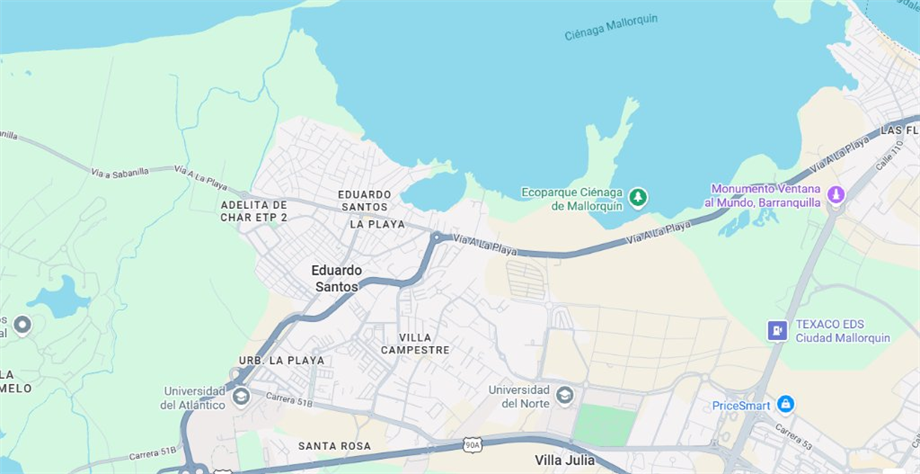
\includegraphics[width=0.78\textwidth]{mapa_barranquilla_google.png}
    \caption{Cartografía base del corredor Circunvalar--Uninorte--Villa Campestre--Arroyo León--Ciénaga de Mallorquín empleada en la aplicación de escritorio (\texttt{interfaz\_app.py}).}
    \label{fig:mapa_google}
\end{figure}

\begin{figure}[H]
    \centering
    \singlespacing
    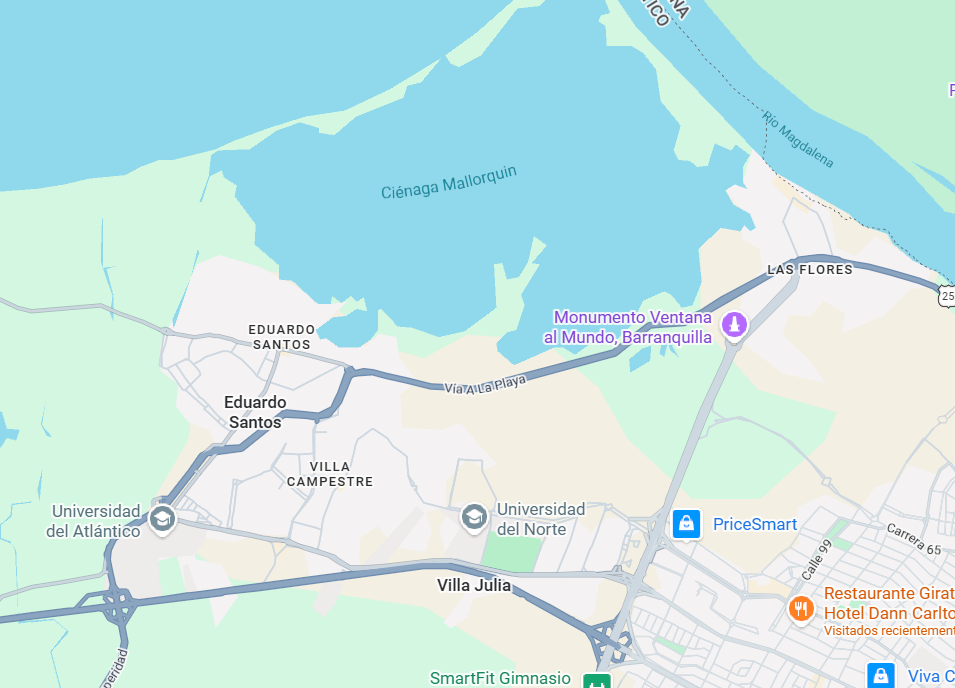
\includegraphics[width=0.78\textwidth]{mapa_panoramico_uninorte.png}
    \caption{Vista panorámica del sector Vía a la Playa--Eduardo Santos--Universidad del Norte utilizada en el prototipo interactivo de validación.}
    \label{fig:mapa_panoramico}
\end{figure}

\subsection{Verificación Automatizada mediante Pruebas Unitarias}

La suite \texttt{test\_arroyos.py} contiene $14$ pruebas unitarias formales (\texttt{unittest}) que verifican la totalidad y determinismo de la tabla de transición de estados, el consenso booleano, las vecindades y el lema del apretón de manos, la bipartición, el subgrafo inducido $G - N_7$, las cotas de planaridad, los recorridos BFS/DFS, la igualdad de costo en Kruskal/Prim ($5\,770\text{ m}$), las centralidades de Unidad 4 y los desvíos seguros de Dijkstra. Tras la versión final del repositorio, la ejecución de \texttt{python -m unittest test\_arroyos.py -v} finalizó con estado \texttt{OK} ($14/14$ pruebas aprobadas en $0.012\text{ s}$).

% ============================================================================
% 6. CONCLUSIONES Y LIMITACIONES
% ============================================================================
\section{Conclusiones y Limitaciones}

\subsection{Conclusiones}

El desarrollo de este proyecto demuestra que las herramientas abstractas de Matemáticas Discretas poseen aplicación directa e inmediata en problemas reales de ingeniería urbana en Barranquilla. Modelar la cuenca hidráulica como un DAG y las vías alternas como un grafo no dirigido permitió unificar en una misma base matemática la propagación preventiva por BFS y el desvío vehicular seguro mediante Dijkstra sobre subgrafos inducidos. Asimismo, la introducción del consenso booleano basado en conjuntos $C(R_v, k)$ resuelve formalmente la incertidumbre propia del reporte ciudadano colaborativo, mientras que las métricas de centralidad e intermediación de la Unidad 4 identifican de forma objetiva qué intersecciones (como $N_7$ y $N_4$) requieren mayor prioridad en infraestructura de drenaje y monitoreo. Todo el código fuente y las instrucciones de reproducción se encuentran documentados y accesibles en \url{https://github.com/Andrestcrack/Proyecto-arroyo}.

\subsection{Limitaciones y Trabajo Futuro}

A pesar de los resultados satisfactorios en simulación y verificación unitaria, el prototipo actual presenta cuatro limitaciones claramente delimitadas:
\begin{enumerate}[leftmargin=2.0cm]
    \item \textbf{Ausencia de telemetría IoT en tiempo real:} La activación de eventos depende actualmente de reportes simulados por usuarios en la interfaz de escritorio o web, sin integración directa con sensores ultrasónicos de nivel de agua o estaciones pluviométricas del IDEAM.
    \item \textbf{Granularidad de la red vial:} Aunque el servidor web incorpora $25$ nodos y $31$ corredores arteriales principales de Barranquilla, las calles barriales secundarias fuera de los ejes troncales no poseen nodos de control hidrológico propio.
    \item \textbf{Dependencia de conectividad para OSRM dinámico:} Aunque existen $71$ corredores viales precargados en caché local para asegurar la operación sin Internet, el cálculo de trazados calle por calle entre coordenadas arbitrarias fuera de los corredores precargados requiere acceso al servicio público OSRM.
    \item \textbf{Persistencia temporal:} Los estados se gestionan en memoria durante la sesión del servidor HTTP, por lo que como trabajo futuro se propone acoplar una base de datos espacial (PostGIS), modelos probabilísticos de lluvia y notificaciones móviles en tiempo real.
\end{enumerate}

% ============================================================================
% 7. REFERENCIAS EN NORMAS APA (7.ª EDICIÓN)
% ============================================================================
\newpage
\section{Referencias}

\begin{singlespacing}
\setlength{\parindent}{0pt}
\everypar{\hangindent=1.27cm \hangafter=1}

Área Metropolitana de Barranquilla. (2021). \textit{Plan Maestro de Drenaje Pluvial y Control de Arroyos Urbanos en el Distrito de Barranquilla y Área Metropolitana}. Alcaldía Distrital de Barranquilla.

Bondy, J. A., \& Murty, U. S. R. (2008). \textit{Graph theory} (Graduate Texts in Mathematics, Vol. 244). Springer. \url{https://doi.org/10.1007/978-1-84628-970-5}

Cormen, T. H., Leiserson, C. E., Rivest, R. L., \& Stein, C. (2022). \textit{Introduction to algorithms} (4.ª ed.). MIT Press.

Dijkstra, E. W. (1959). A note on two problems in connexion with graphs. \textit{Numerische Mathematik}, \textit{1}(1), 269--271. \url{https://doi.org/10.1007/BF01386390}

Kruskal, J. B. (1956). On the shortest spanning subtree of a graph and the traveling salesman problem. \textit{Proceedings of the American Mathematical Society}, \textit{7}(1), 48--50. \url{https://doi.org/10.1090/S0002-9939-1956-0078686-7}

Newman, M. E. J. (2018). \textit{Networks} (2.ª ed.). Oxford University Press. \url{https://doi.org/10.1093/oso/9780198805090.001.0001}

OpenStreetMap Contributors \& Project OSRM. (2026). \textit{Open Source Routing Machine: Modern C++ routing engine for shortest paths in road networks}. \url{https://project-osrm.org/}

Prim, R. C. (1957). Shortest connection networks and some generalizations. \textit{Bell System Technical Journal}, \textit{36}(6), 1389--1401. \url{https://doi.org/10.1002/j.1538-7305.1957.tb01515.x}

Python Software Foundation. (2026). \textit{The Python Standard Library: tkinter, http.server, heapq y unittest} (Versión 3.15). \url{https://docs.python.org/3/library/}

Rosen, K. H. (2021). \textit{Discrete mathematics and its applications} (8.ª ed.). McGraw-Hill Education.

\end{singlespacing}

\end{document}
